\begin{enumerate}[label=\bfseries Câu \arabic*:]
	
\item \mkstar{1}

\cauhoi{Khi tần số dòng điện xoay chiều chạy qua đoạn mạch chỉ chứa cuộn cảm tăng lên 4 lần thì cảm kháng của cuộn cảm
	\begin{mcq}(2)
		\item tăng lên 2 lần.
		\item tăng lên 4 lần.
		\item giảm đi 4 lần.
		\item giảm đi 2 lần.
	\end{mcq}
}	
	\loigiai{
		\textbf{Đáp án: B.}
		
		Khi tần số dòng điện xoay chiều chạy qua đoạn mạch chỉ chứa cuộn cảm tăng lên 4 lần thì cảm kháng của cuộn cảm sẽ tăng lên 4 lần.
		
		}

%%%%%%%%%%%%%%CÂU2%%%%%%%%%%
\item \mkstar{1}

\cauhoi{Phát biểu nào sau đây là \textbf{không} đúng?
	\begin{mcq}(1)
		\item Công suất của dòng điện xoay chiều phụ thuộc vào công suất hao phí trên đường dây tải điện.
		\item Công suất của dòng điện xoay chiều phụ thuộc vào hiệu điện thế hiệu dụng giữa hai đầu đoạn mạch.
		\item Công suất của dòng điện xoay chiều phụ thuộc vào cường độ dòng điện hiệu dụng trong mạch.
		\item Công suất của dòng điện xoay chiều phụ thuộc vào bản chất của mạch điện và tần số dòng điện trong mạch.
	\end{mcq}
}	
	\loigiai{
		\textbf{Đáp án: A.}
		
		Công suất của dòng điện xoay chiều được tính theo công thức $P=UI\cos\varphi$. Suy ra công suất của dòng điện xoay chiều phụ thuộc vào cường độ dòng điện hiệu dụng I trong mạch, điện áp hiệu dụng U giữa hai đầu đoạn mạch, bản chất của mạch điện và tần số dòng điện trong mạch (đặc trưng bởi độ lệch pha).
		
		}

%%%%%%%%%%%%%%CÂU3%%%%%%%%%%
\item \mkstar{1}

\cauhoi{Chọn trả lời \textbf{sai}. Dòng điện xoay chiều là
	\begin{mcq}
		\item dòng điện mà cường độ biến thiên theo dạng sin.
		\item dòng điện đổi chiều một cách tuần hoàn.
		\item dòng điện dao động điều hòa.
		\item dòng điện mà cường độ dòng điện biến thiên theo dạng cos.
	\end{mcq}
}
	\loigiai{
		\textbf{Đáp án: B.}
		
		Dòng điện xoay chiều là dòng điện dao động điều hòa biến thiên theo dạng sin, cos.
		
		}

%%%%%%%%%%%%%%CÂU4%%%%%%%%%%
\item \mkstar{1}

\cauhoi{Công suất của dòng điện xoay chiều trên đoạn mạch RLC nối tiếp \textbf{không} phụ thuộc vào đại lượng nào sau đây?
	\begin{mcq}
		\item Hiệu điện thế cực đại giữa hai đầu đoạn mạch.
		\item Cường độ hiệu đụng của dòng điện qua mạch.
		\item Độ lệch pha giữa dòng điện và hiệu điện thế giữa hai bản tụ.
		\item Tỉ số giữa điện trở thuần và tổng trở của mạch.
	\end{mcq}
}	
	\loigiai{
		\textbf{Đáp án: C.}
		
		Độ lệch pha giữa dòng điện và điện áp giữa hai đầu tụ điện luôn là $\dfrac{\pi}{2}$.
		
		}

%%%%%%%%%%%%%%CÂU5%%%%%%%%%%
\item \mkstar{1}

\cauhoi{Chọn phát biểu \textbf{sai}.
	\begin{mcq}
		\item Trong đoạn mạch chỉ chứa điện trở R thì cường độ dòng điện và điện áp hai đầu mạch luôn luôn cùng pha nhau.
		\item Trong đoạn mạch chỉ có cuộn dây thuần cảm kháng, dđiện luôn chậm pha hơn điện áp tức thời một góc $90^\circ$.
		\item Cường độ dòng điện qua cuộn dây $I_0=U_0L/Z_L$.
		\item Cường độ dòng điện qua mạch điện $I_0=U/R$.
	\end{mcq}
}	
	\loigiai{
		\textbf{Đáp án: D.}
		
		Cường độ dòng điện qua mạch điện $I_0=U/Z$.
		
		}

%%%%%%%%%%%%%%CÂU6%%%%%%%%%%
\item \mkstar{1}

\cauhoi{Chọn câu đúng.
	\begin{mcq}
		\item Dung kháng của tụ điện tỉ lệ nghịch với chu kỳ của dòng điện xoay chiều.
		\item Hiệu điện thế giữa hai bản tụ biến thiên sớm pha $\pi/2$ đối với dòng điện.
		\item Cường độ hiệu dụng của dòng điện xoay chiều qua tụ điện tỉ lệ nghịch với tần số dòng điện.
		\item Tụ điện cho cả dòng điện xoay chiều và dòng điện một chiều đi qua.
	\end{mcq}
}
	\loigiai{
		\textbf{Đáp án: A.}
		
		Dung kháng của tụ điện tỉ lệ nghịch với chu kỳ của dòng điện xoay chiều.
		
		}

%%%%%%%%%%%%%%CÂU7%%%%%%%%%%
\item \mkstar{1}

\cauhoi{Trong các dụng cụ tiêu thụ điện như quạt, tủ lạnh, động cơ, người ta nâng cao hệ số công suất nhằm
	\begin{mcq}(2)
		\item tăng cường độ dòng điện.
		\item tăng công suất tiêu thụ.
		\item giảm cường độ dòng điện.
		\item giảm công suất tiêu thụ.
	\end{mcq}
}	
	\loigiai{
		\textbf{Đáp án: C.}
		
		Trong các dụng cụ tiêu thụ điện như quạt, tủ lạnh, động cơ, người ta năng cao hệ số công suất nhằm giảm cường độ dòng điện, giảm hao phí tỏa nhiệt và nâng cao hiệu suất.
		
		}

%%%%%%%%%%%%%%CÂU8%%%%%%%%%%
\item \mkstar{1}

\cauhoi{Công suất tỏa nhiệt trong mỗi mạch điện phụ thuộc vào
	\begin{mcq}(2)
		\item các thành phần cấu tạo nên mạch.
		\item cảm kháng.
		\item điện trở.
		\item dung kháng.
	\end{mcq}
}
	\loigiai{
		\textbf{Đáp án: C.}
		
		Công suất tỏa nhiệt của một mạch điện xoay chiều phụ thuộc vào điện trở của mạch.
		
		}

%%%%%%%%%%%%%%CÂU9%%%%%%%%%%
\item \mkstar{2}

\cauhoi{Đặt điện áp $u=90\sqrt{2}\cos \left( 100\pi t-\dfrac{\pi}{2} \right)\text{ (V)}$ vào hai đầu một đoạn mạch gồm điện trở thuần $R=30\ \Omega$ mắc nối tiếp với một cuộn cảm thuần có độ tự cảm $L=50\cdot\dfrac{10^{-2}}{\pi} \text{ H}$  và tụ điện có điện dung $C=5\cdot\dfrac{10^{-4}}{\pi} \text{ F}$. Viết biểu thức cường độ dòng điện trong mạch.
	\begin{mcq}(2)
		\item $i=3\cos \left( 100\text{ }\!\!\pi\!\!\text{ t}-\dfrac{3\text{ }\!\!\pi\!\!\text{ }}{4} \right)\text{ }\!\!~\!\!\text{ A}.$
		\item $i=3\cos \left( 100\text{ }\!\!\pi\!\!\text{ t}-\dfrac{5\text{ }\!\!\pi\!\!\text{ }}{4} \right)\text{ }\!\!~\!\!\text{ A}.$
		\item $i=4\cos \left( 100\text{ }\!\!\pi\!\!\text{ t}-\dfrac{3\text{ }\!\!\pi\!\!\text{ }}{4} \right)\text{ }\!\!~\!\!\text{ A}.$
		\item $i=4\cos \left( 100\text{ }\!\!\pi\!\!\text{ t}-\dfrac{5\text{ }\!\!\pi\!\!\text{ }}{4} \right)\text{ }\!\!~\!\!\text{ A}.$
	\end{mcq}
}	
\loigiai{
	\textbf{Đáp án: A.}
	
	Tổng trở của mạch:
	$$Z=\sqrt{R^2+(Z_L-Z_C)^2}=30\sqrt{2}\,\Omega.$$
	Cường độ dòng điện cực đại:
	$$I_0=\dfrac{{U_{0}}}{Z}=3\text{ }\!\!~\!\!\text{ A}.$$
	Pha ban đầu của cường độ dòng điện:
	$$\tan \text{ }\!\!\varphi\!\!\text{ }=\dfrac{{Z_L}-Z_C}{R}=1\Rightarrow \text{ }\!\!\varphi\!\!\text{ }=\dfrac{\text{ }\!\!\pi\!\!\text{ }}{4}~\text{rad}.$$
	$$\Rightarrow{{\text{ }\!\!\varphi\!\!\text{ }}_{\text{i}}}={{\text{ }\!\!\varphi\!\!\text{ }}_{\text{u}}}-\text{ }\!\!\varphi\!\!\text{ }=-\dfrac{3\text{ }\!\!\pi\!\!\text{ }}{4}\text{ }\!\!~\!\!\text{ rad}.$$
	Biểu thức cường độ dòng điện trong mạch:
	$$i=3\cos \left( 100\text{ }\!\!\pi\!\!\text{ t}-\dfrac{3\text{ }\!\!\pi\!\!\text{ }}{4} \right)\text{ }\!\!~\!\!\text{ A}.$$
	
}
\item \mkstar{2}

\cauhoi{Cho đoạn mạch gồm điện trở thuần $R = 40\ \Omega$, tụ điện có $C = \dfrac{10^{-3}}{6\pi}\ \si{\farad}$ và cuộn dây thuần cảm có $L = \dfrac{1}{\pi}\ \si{\farad}$ mắc nối tiếp. Điện áp hai đầu mạch $u = 120 \cos (100 \pi t + \dfrac{\pi} {3})\ \textrm{(V).}$ Biểu thức cường độ dòng điện trong mạch:
	
	\begin{mcq}(2)
		\item $i=\text{1,5}\sqrt{2}\cos \left( 100\text{ }\!\!\pi\!\!\text{ t}-\dfrac{\text{ }\!\!\pi\!\!\text{ }}{12} \right)\text{ }\!\!~\!\!\text{ A}.$
		\item $i=\text{1,5}\sqrt{2}\cos \left( 100\text{ }\!\!\pi\!\!\text{ t}+\dfrac{\text{ }\!\!\pi\!\!\text{ }}{12} \right)\text{ }\!\!~\!\!\text{ A}.$
		\item $i=3\cos \left( 100\text{ }\!\!\pi\!\!\text{ t}-\dfrac{\text{ }\!\!\pi\!\!\text{ }}{12} \right)\text{ }\!\!~\!\!\text{ A}.$
		\item $i=3\cos \left( 100\text{ }\!\!\pi\!\!\text{ t}+\dfrac{\text{ }\!\!\pi\!\!\text{ }}{12} \right)\text{ }\!\!~\!\!\text{ A}.$
	\end{mcq}	
}	
\loigiai{
	\textbf{Đáp án: B.}
	
	Tổng trở của mạch:
	$$Z=\sqrt{R^2+(Z_L-Z_C)^2}=40\sqrt{2}\,\Omega.$$
	Dòng điện cực đại:
	$$I_0=\dfrac{{U_{0}}}{Z}=1,5\sqrt{2}\text{ }\!\!~\!\!\text{ A}.$$
	Pha ban đầu:
	$$\tan \text{ }\!\!\varphi\!\!\text{ }=\dfrac{{Z_L}-Z_C}{R}=1\Rightarrow \text{ }\!\!\varphi\!\!\text{ }=\dfrac{\text{ }\!\!\pi\!\!\text{ }}{4}~\text{rad}.$$
	$$\Rightarrow{{\text{ }\!\!\varphi\!\!\text{ }}_{\text{i}}}={{\text{ }\!\!\varphi\!\!\text{ }}_{\text{u}}}-\text{ }\!\!\varphi\!\!\text{ }=\dfrac{\text{ }\!\!\pi\!\!\text{ }}{12}\text{ }\!\!~\!\!\text{ rad}.$$
	Biểu thức cường độ dòng điện trong mạch:
	$$i=1,5\sqrt{2}\cos \left( 100\text{ }\!\!\pi\!\!\text{ t}+\dfrac{\text{ }\!\!\pi\!\!\text{ }}{12} \right)\text{ }\!\!~\!\!\text{ A}.$$
	
}
\item \mkstar{2}

\cauhoi{Trên đoạn mạch xoay chiều $RLC$ mắc nối tiếp. Điện trở thuần $R=\SI{10}{\ohm}$. Cuộn dây thuần cảm có độ tự cảm $L=\dfrac{1}{10\pi}\,\text{H}$, tụ điện có điện dung $C$ thay đổi được. Mắc vào hai đầu đoạn mạch có điện áp xoay chiều $u=U_0\cos(100\pi t)\,\text{V}$. Để điện áp giữa hai đầu đoạn mạch cùng pha với điện áp giữa hai đầu điện trở $R$ thì điện dung của tụ điện là
	\begin{mcq}(4)
		\item $C=\dfrac{10^{-3}}{\pi}\,\text{F}$.
		\item $C=\dfrac{10^{-4}}{2\pi}\,\text{F}$.
		\item $C=\dfrac{10^{-4}}{\pi}\,\text{F}$.
		\item $C=\SI{3,18}{\micro\farad}$.
	\end{mcq}
}	
	\loigiai{
		\textbf{Đáp án: A.}
		
		Để điện áp giữa hai đầu đoạn mạch cùng pha với điện áp giữa hai đầu điện trở $R$ thì xảy ra cộng hưởng, điện dung của tụ điện là	
		$$Z_L=Z_C\Rightarrow C=\dfrac{10^{-3}}{\pi}\,\text{F}$$
		
		}

%%%%%%%%%%%%%%CÂU10%%%%%%%%%%
\item \mkstar{2}

\cauhoi{Dòng điện xoay chiều trong đoạn mạch $RLC$ có tần số $\SI{50}{Hz}$, cuộn cảm thuần $L=\dfrac{1}{4\pi}\,\text{H}$. Tụ điện có điện dung biến thiên đang được điều chỉnh ở giá trị $C_1=\dfrac{4}{\pi}\cdot 10 ^{-4}\,\text{F}$. Điện trở thuần $R$ không đổi. Tăng dần điện dung của tụ điện từ giá trị $C_1$ cường độ hiệu dụng của dòng điện sẽ
	\begin{mcq}(2)
		\item lúc đầu tăng sau đó giảm.
		\item tăng.
		\item giảm.
		\item lúc đầu giảm sau đó tăng.
	\end{mcq}
}	
	\loigiai{
		\textbf{Đáp án: C.}
		
		Ta có $Z_L=Z_C=\SI{25}{\ohm}$.
		
		Mạch xảy ra cộng hưởng nên nếu tăng dần điện dung thì cường độ dòng điện giảm.
		
	}

%%%%%%%%%%%%%%CÂU11%%%%%%%%%%
\item \mkstar{2}

\cauhoi{Lần lượt đặt vào hai đầu một đoạn mạch $RLC$ mắc nối tiếp các điện áp $u_1$, $u_2$, $u_3$ có cùng giá trị hiệu dụng nhưng tần số khác nhau, cường độ dòng điện trong mạch tương ứng là $i_1=I_0\cos 100\pi t$, $i_2=I_0\cos(120\pi t+2\pi/3)$, $i_3=I\sqrt{2}\cos(110\pi t-2\pi/3)$. Hệ thức nào sau đây đúng?
	\begin{mcq}(4)
		\item $I>I_0/\sqrt{2}$.
		\item $I<I_0/\sqrt{2}$.
		\item $I<I_0/\sqrt{3}$.
		\item $I=I_0/\sqrt{2}$.
	\end{mcq}
}	
	\loigiai{
	\textbf{Đáp án: A.}
		
		Vì $I_{01}=I_{02}=I_0\Rightarrow \omega_1\omega_2=\omega_3^2\Rightarrow I>I_0/\sqrt{2}$
		
		}

%%%%%%%%%%%%%%CÂU12%%%%%%%%%%
\item \mkstar{2}

\cauhoi{Đoạn mạch xoay chiều gồm điện trở thuần $R=\SI{100}{\ohm}$, cuộn dây thuần cảm $L=\dfrac{1}{\pi}\,\text{H}$ và tụ C thay đổi được. Đặt vào hai đầu mạch điện áp có giá trị hiệu dụng $\SI{200}{V}$, tần số $\SI{50}{Hz}$. Thay đổi $C$ đến khi điện áp giữa hai đầu cuộn dây đạt giá trị cực đại, giá trị cực đại đó bằng
	\begin{mcq}(4)
		\item $\SI{200}{V}$.
		\item $\SI{100}{V}$.
		\item $\SI{300}{V}$.
		\item $\SI{150}{V}$.
	\end{mcq}
}	
	\loigiai{
		\textbf{Đáp án: A.}
		
		Khi $C$ thay đổi để $U_{L\textrm{ max}}$ thì có cộng hưởng điện
		
		Khi đó $Z_L=Z_C=\SI{100}{\ohm}$.
		
		Điện áp $U_L=\dfrac{U}{R}Z_L=\SI{200}{V}$.
		
	}

%%%%%%%%%%%%%%CÂU13%%%%%%%%%%
\item \mkstar{2}

\cauhoi{Đặt vào hai đầu đoạn mạch $RLC$ mắc nối tiếp một hiệu điện thế dao động điều hòa có biểu thức $u=220\sqrt{2}\cos\omega t\,\text{V}$. Biết điện trở thuần của mạch có giá trị là $\SI{100}{\ohm}$. Khi $\omega$ thay đổi thì công suất tiêu thụ cực đại của mạch có giá trị là
	\begin{mcq}(4)
		\item $\SI{440}{\watt}$.
		\item $\SI{484}{\watt}$.
		\item $\SI{220}{\watt}$.
		\item $\SI{242}{\watt}$.
	\end{mcq}
}	
	\loigiai{
	\textbf{Đáp án: B.}
		
		Khi $\omega$ thay đổi để $P_\text{max}$ thì hiện tượng cộng hưởng xảy ra
		$$P_\text{max}=\dfrac{U^2}{R}=\SI{484}{\watt}.$$
		
		}
\item \mkstar{2}

\cauhoi{Mắc mạch điện xoay chiều $R$, $L$, $C$ nối tiếp vào điện áp $u=U_0 \cos \left(100 \pi t + \dfrac{\pi}{2}\right)\ \text{(V)}$ thì dòng điện qua mạch là $i=I_0 \cos \left(100 \pi t + \dfrac{\pi}{6} \right)\ \text{(A)}$. Kết luận nào sau đây đúng? 
	\begin{mcq}(4)
		\item $Z_L < Z_C$.
		\item $Z_L=Z_C$.
		\item $Z_L > Z_C$.
		\item $Z_L < R$.
	\end{mcq}
}	
\loigiai{
	\textbf{Đáp án: C.}
	
	Mạch điện gồm $R$, $L$, $C$ mắc nối tiếp.
	
	Mối liên hệ về pha giữa $u$ và $i$:
	
	\begin{equation*} \varphi_u = \dfrac{\pi}{2}\ \text{rad} > \varphi_i = \dfrac{\pi}{6}\ \text {rad},
	\end{equation*}
	suy ra $u$ nhanh pha hơn $i$.
	
	Vậy mạch có tính cảm kháng: $Z_L > Z_C$.
	
}
%%%%%%%%%%%%%%CÂU14%%%%%%%%%%
\item \mkstar{2}

\cauhoi{Cho mạch điện xoay chiều $RLC$ (cuộn dây thuần cảm). Đặt vào hai đầu đoạn mạch điện áp xoay chiều có giá trị hiệu dụng $U=\SI{120}{V}$ và tần số $f$ xác định. Biết $CR^2=16L$ và điện áp giữa hai đầu đoạn mạch vuông pha với điện áp giữa hai đầu tụ điện. Điện áp giữa hai đầu tụ điện và hai đầu cuộn cảm là
	\begin{mcq}(2)
		\item $U_C=U_L=\SI{60}{V}$.
		\item $U_C=\SI{30}{V}$ và $U_L=\SI{60}{V}$.
		\item $U_C=U_L=\SI{30}{V}$.
		\item $U_C=\SI{60}{V}$ và $U_L=\SI{30}{V}$.
	\end{mcq}
}	
	\loigiai{
			\textbf{Đáp án: C.}
		
		Ta có $CR^2=16L\Rightarrow R^2=16Z_LZ_C$.
		
		Khi $u$ vuông góc với $u_C$ thì $u$ và $i$ cùng pha nhau nên có cộng hưởng điện $Z_L=Z_C$. Do đó $R=4Z_L$.
		
		Theo bài ra $U_R=U=\SI{120}{V}$ nên $U_C=U_L=\SI{30}{V}$.
		
	}
\item \mkstar{2}

\cauhoi{Đặt điện áp $u=U_0 \cos \omega t$ ($U_0$ không đổi, $\omega$ thay đổi được) vào hai đầu đoạn mạch gồm điện trở $R$, cuộn cảm thuần có độ tự cảm $L$ và tụ điện có điện dung $C$ mắc nối tiếp. Hiện tượng cộng hưởng điện xảy ra khi
	\begin{mcq}(2)
		\item $\omega^2 LCR - 1 = 0$.
		\item $R=\left|\omega L - \dfrac{1}{\omega C}\right|$.
		\item $\omega^2 LC -1 =0$.
		\item $\omega^2 LC - R = 0$.
	\end{mcq}
}	
\loigiai{
	\textbf{Đáp án: C.}
	
	Khi xảy ra hiện tượng cộng hưởng điện:
	\begin{equation*}
		Z_L = Z_C \Leftrightarrow \omega L =\dfrac{1}{\omega C} \Leftrightarrow \omega ^2 = \dfrac{1}{LC} \Leftrightarrow \omega^2 LC -1 =0.
	\end{equation*}
	
}
\item \mkstar{2}

\cauhoi{Cho mạch điện xoay chiều gồm điện trở $R$, cuộn cảm thuần có độ tự cảm $L=\dfrac{0,2}{\pi}\, \text{H}$ và tụ điện có điện dung $C=\dfrac{5\cdot 10^{-4}}{\pi}\, \text{F}$. Tính giá trị tần số góc $\omega$ để trong mạch có cộng hưởng điện.
	\begin{mcq}(2)
		\item $100\pi~\text{rad/s}$.
		\item $50\pi~\text{rad/s}$.
		\item $100~\text{rad/s}$.
		\item $50~\text{rad/s}$.
	\end{mcq}
}	
\loigiai{
	\textbf{Đáp án: A.}
	
	Cộng hưởng điện xảy ra khi $Z_L=Z_C$ hay $\omega^2LC=1$.
	
	
	Vậy tần số góc $\omega= \dfrac{1}{\sqrt{LC}}=100\pi\, \textrm{rad/s}.$
	
}
\item \mkstar{2}

\cauhoi{Đặt điện áp xoay chiều $u=U \sqrt 2 \cos 100 \pi t\ \text{(V)}$ ($t$ tính bằng $\SI{}{\second}$) vào hai đầu đoạn mạch có $R$, $L$, $C$ mắc nối tiếp thì có cộng hưởng điện. Biết cuộn cảm có cảm kháng $\SI{80}{\Omega}$. Điện dung của tụ điện có giá trị là
	\begin{mcq}(4)
		\item $\SI{0.25}{\farad}$.
		\item $\SI{1.25e-4}{\farad}$.
		\item $\SI{3.98e-5}{\farad}$.
		\item $\SI{0.80}{\farad}$.
	\end{mcq}
}	
\loigiai{
	\textbf{Đáp án: C.}
	
	Khi xảy ra hiện tượng cộng hưởng điện:
	\begin{equation*}
		Z_L = Z_C \Leftrightarrow Z_L = \dfrac{1}{\omega C} \Leftrightarrow C  = \dfrac{1}{\omega Z_L} \approx \SI{3.98e-5}{\farad}.
	\end{equation*}
	
}
\item \mkstar{3}

\cauhoi{Đặt một điện áp xoay chiều có giá trị hiệu dụng không đổi lần lượt vào hai đầu đoạn mạch chỉ có điện trở $R$, cuộn cảm thuần $L$ hoặc tụ điện $C$ thì cường độ dòng điện hiệu dụng chạy qua các phần tử lần lượt là $4~\text{A}$, $6~\text{A}$ và $2~\text{A}$. Nếu đặt điện áp đó vào đoạn mạch gồm cả ba phần tử trên mắc nối tiếp thì cường độ dòng điện hiệu dụng qua mạch là bao nhiêu?
	\begin{mcq}(4)
		\item $\text{2,2}~\text{A}$.
		\item $\text{2,4}~\text{A}$.
		\item $\text{2,6}~\text{A}$.
		\item $\text{2,8}~\text{A}$.
	\end{mcq}		
}	
\loigiai{
	\textbf{Đáp án: B.}
	
	Cường độ dòng hiệu dụng qua mạch chỉ có $R$: $${{I}_{1}}=U/R=4~\text{A}.$$
	Cường độ dòng hiệu dụng qua mạch chỉ có $L$: $${{I}_{2}}=U/Z_L=6~\text{A}.$$
	Cường độ dòng hiệu dụng qua mạch chỉ có $C$: $${{I}_{3}}=U/Z_C=2~\text{A}.$$
	Cường độ dòng điện hiệu dụng qua mạch $RLC$:
	$$I=\dfrac{U}{Z}=\dfrac{U}{\sqrt{{{R}^{2}}+{{\left( {{Z}_{L}}-{{Z}_{C}} \right)}^{2}}}}=\dfrac{U}{\sqrt{{{\left( \dfrac{U}{{{I}_{1}}} \right)}^{2}}+{{\left( \dfrac{U}{{{I}_{2}}}-\dfrac{U}{{{I}_{3}}} \right)}^{2}}}}=\text{2,4}~\text{A}.$$
	
}
%%%%%%%%%%%%%%CÂU15%%%%%%%%%%
\item \mkstar{3}

\cauhoi{Cho đoạn mạch không phân nhánh $RLC$, $R=\SI{80}{\ohm}$,cuộn dây có điện trở trong $\SI{20}{\ohm}$ và độ tự cảm $L=\SI{0,318}{H}$, tụ điện có điện dung $\SI{15,9}{\micro\farad}$. Đặt vào hai đầu mạch điện một dòng điện xoay chiều có tần số $f$ thay đổi được có hiệu điện thế hiệu dụng là $\SI{200}{V}$.Khi công suất trên toàn mạch đạt giá trị cực đại thì giá trị của $f$ và $\calP$ bằng bao nhiêu?
	\begin{mcq}(2)
		\item $\SI{70,78}{Hz}$ và $\SI{400}{\watt}$.
		\item $\SI{70,78}{Hz}$ và $\SI{500}{\watt}$.
		\item $\SI{444,7}{Hz}$ và $\SI{2000}{\watt}$.
		\item $\SI{31,48}{Hz}$ và $\SI{400}{\watt}$.
	\end{mcq}
}	
	\loigiai{
			\textbf{Đáp án: A.}
		
		Khi cường độ dòng điện trong mạch cực đại thì cộng hưởng điện xảy ra. Khi đó cường độ dòng điện cực đại là
		$$I=\dfrac{U}{R+r}=\SI{2}{A}.$$
		
		Tần số dòng điện là
		$$f=\dfrac{\omega}{2\pi}=\dfrac{1}{2\pi\sqrt{LC}}=\SI{70,78}{Hz}.$$
		
		Công suất cực đại là $P=I^2(R+r)=\SI{400}{\watt}$.
		
	}

%%%%%%%%%%%%%%CÂU16%%%%%%%%%%
\item \mkstar{3}

\cauhoi{Đặt vào hai đầu đoạn mạch $RLC$ mắc nối tiếp một hiệu điện thế dao động điều hòa có biểu thức $u=220\cos\omega t\, \text{V}$. Khi $\omega$ thay đổi công suất tiêu thụ cực đại của mạch là $\SI{484}{\watt}$. Khi đó điện trở thuần của mạch là
	\begin{mcq}(4)
		\item $R=\SI{50}{\ohm}$.
		\item $R=\SI{750}{\ohm}$.
		\item $R=\SI{150}{\ohm}$.
		\item $R=\SI{100}{\ohm}$.
	\end{mcq}
}	
	\loigiai{
			\textbf{Đáp án: A.}
		
		Khi $\omega$ thay đổi để công suất cực đại thì có cộng hưởng. Điện trở thuần của mạch là
		$$R=\dfrac{U^2}{P}=\SI{50}{\ohm}.$$
		
	}

%%%%%%%%%%%%%%CÂU17%%%%%%%%%%
\item \mkstar{3}

\cauhoi{Đoạn mạch xoay chiều gồm điện trở $R$, tụ điện có điện dung $C$ thay đổi được, cuộn dây có độ tự cảm $L=\dfrac{1}{\pi}\,\text{H}$ và điện trở $r=\SI{20}{\ohm}$ mắc nối tiếp. Đặt vào hai đầu đoạn mạch điện áp xoay chiều có giá trị hiệu dụng $U=\SI{60}{V}$ và tần số $f=\SI{50}{Hz}$. Điều chỉnh điện dung tụ điện đến giá trị $C_1$ thì công suất tiêu thụ trên mạch đạt cực đại và bằng $\SI{30}{\watt}$. Điện trở $R$ và điện dung $C_1$ có giá trị là
	\begin{mcq}(2)
		\item $R=\SI{120}{\ohm}$; $C_1=\dfrac{10^4}{2\pi}\,\text{F}$.
		\item $R=\SI{120}{\ohm}$; $C_1=\dfrac{10^4}{\pi}\,\text{F}$.
		\item $R=\SI{100}{\ohm}$; $C_1=\dfrac{10^4}{2\pi}\,\text{F}$.
		\item $R=\SI{100}{\ohm}$; $C_1=\dfrac{10^4}{\pi}\,\text{F}$.
	\end{mcq}
}	
	\loigiai{
			\textbf{Đáp án: D.}
		
		Khi $C$ thay đổi để công suất cực đại thì xảy ra hiện tượng cộng hưởng nên $C=\dfrac{10^4}{\pi}\,\text{F}$.
		
		Điện trở là $R=\dfrac{U^2}{P_\text{max}}-r=\SI{100}{\ohm}$.
		
	}
\item \mkstar{3}

\cauhoi{Đặt điện áp xoay chiều $u=60\sqrt 2 \cos 100 \pi t \ \text{(V)}$ ($t$ tính bằng $\SI{}{\second}$) vào hai đầu đoạn mạch mắc nối tiếp gồm điện trở $\SI{30}{\Omega}$, tụ điện có điện dung $\dfrac{10^{-3}}{4\pi}\ \text F$ và cuộn cảm thuần có độ tự cảm $L$ thay đổi được. Điều chỉnh $L$ để cường độ hiệu dụng của dòng điện trong mạch đạt cực đại. Khi đó, điện áp hiệu dụng giữa hai đầu cuộn cảm là
	\begin{mcq}(4)
		\item $\SI{80}{\volt}$.
		\item $80\sqrt2\ \text V$.
		\item $60\sqrt2\ \text V$.
		\item $60\ \text V$.
	\end{mcq}
}	
\loigiai{
	\textbf{Đáp án: A.}
	
	Khi xảy ra hiện tượng cộng hưởng điện, cường độ dòng điện hiệu dụng trong mạch đạt cực đại:
	\begin{equation*}
		I=\dfrac{U}{R}=\SI{2}{\ampere}.
	\end{equation*}
	
	Ngoài ra, cảm kháng $Z_L$ bằng dung kháng $Z_C$, suy ra \begin{equation*}
		Z_L=Z_C=\dfrac{1}{\omega C} = \SI{40}{\Omega}.
	\end{equation*}
	
	Điện áp hiệu dụng giữa hai đầu cuộn cảm:
	\begin{equation*}
		U_L = I Z_L = \SI{80}{\volt}.
	\end{equation*}
	
}
%%%%%%%%%%%%%%CÂU18%%%%%%%%%%
\item \mkstar{3}

\cauhoi{Cho mạch điện gồm $R$, $L$, $C$ mắc nối tiếp. Biết $R=\SI{30}{\ohm}$, $R=\SI{0,4}{H}$, $C$ thay đổi được. Đặt vào hai đầu mạch điện một hiệu điện thế xoay chiều $u=120\cos(100t+\pi/2)\,\text{V}$. Khi $C=C_0$ thì công suất trong mạch đạt giá trị cực đại. Khi đó biểu thức điện áp giữa hai đầu điện trở là
	\begin{mcq}(2)
		\item $u_R=60\sqrt{2}\cos100t\,\text{V}$.
		\item $u_R=120\sqrt{2}\cos(100t+\pi/2)\,\text{V}$.
		\item $u_R=120\sqrt{2}\cos100t\,\text{V}$.
		\item $u_R=60\sqrt{2}\cos(100t+\pi/2)\,\text{V}$.
	\end{mcq}
}	
	\loigiai{
	\textbf{Đáp án: B.}
		
		Ta có cảm kháng là $Z_L=\omega L=\SI{40}{\omega}$.
		
		Khi $C$ thay đổi để công suất tiêu thụ cực đại thì $Z_L=Z_C=\SI{40}{\ohm}$.
		
		Do đó $u_R$ cùng pha với $u$ nên $u_R=120\sqrt{2}\cos(100t+\pi/2)\,\text{V}$.
		
		}

%%%%%%%%%%%%%%CÂU19%%%%%%%%%%
	\item \mkstar{3}

\cauhoi{Đặt điện áp  $u=100\sqrt 2\cos 100\pi t\ \text{V}$  vào hai đầu đoạn mạch mắc nối tiếp gồm điện trở thuần $R$, cuộn cảm thuần có độ tự cảm $L$ và tụ điện có điện dung $C$ thay đổi được. Thay đổi $C$ để điện áp hiệu dụng giữa hai bản tụ điện đạt cực đại; khi đó điện áp hiệu dụng ở hai đầu cuộn cảm là $U_L =\text{97,5}\ \text{V}$. So với điện áp hai đầu đoạn mạch thì điện áp hai đầu điện trở thuần:
	
	\begin{mcq}(2)
		\item sớm pha hơn một góc $\text{0,22}\pi$.
		\item sớm pha hơn một góc $\text{0,25}\pi$.
		\item trễ pha hơn một góc $\text{0,22}\pi$.
		\item trễ pha hơn một góc $\text{0,25}\pi$.
	\end{mcq}
}	
	\loigiai{
			\textbf{Đáp án: A.}
		
		\begin{center}
			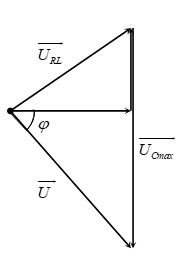
\includegraphics[scale=0.9]{../figs/VN12-PH-19-P-013-1-1.jpg}
		\end{center}
		
		+ Khi $C$ biến thiên để $U_C$  cực đại thì điện áp hai đầu đoạn mạch vuông pha với điện áp hai đầu đoạn mạch $RL$.
		
		+ Từ hình vẽ, ta có: 
		
		$$U^2 = U_{C\text{max}} (U_{C\text{max}} - U_L)  \Rightarrow 100^2  = U_{C\text{max}} (U_{C\text{max}} -\text{97,5}) \Rightarrow U_{C\text{max}} =160\ \text{V}$$
		$$\sin \varphi = \dfrac{U_C- U_L}{U} = \text{0,625} \Rightarrow \varphi = \text{0,22}  \pi$$
		Vậy điện áp hai đầu điện trở sớm pha hơn điện áp hai đầu đoạn mạch một góc $\text{0,22}  \pi$ rad.
		
	}
		\item \mkstar{3}
	
	\cauhoi{Đặt điện áp $u =160\sqrt 2\cos 100\pi t\ \text{V}$ vào hai đầu đoạn mạch mắc nối tiếp gồm điện trở $R=40\sqrt 3\ \Omega$ tụ điện và cuộn cảm thuần có độ tự cảm $L$ thay đổi được. Điều chỉnh độ tự cảm đến giá trị $L=L_0$ để điện áp hiệu dụng hai đầu cuộn cảm đạt giá trị cực đại và bằng 320 V. Biểu thức cường độ dòng điện trong mạch khi đó là
		\begin{mcq}(2)
			\item $i = 2\cos \left(100\pi t -\dfrac{\pi}{3}\right)\ \text{A}$.
			\item $i = 4\cos \left(100\pi t -\dfrac{\pi}{3}\right)\ \text{A}$.
			\item $i = 4\sqrt 2\cos \left(100\pi t -\dfrac{\pi}{6}\right)\ \text{A}$.
			\item $i = 2\sqrt 2\cos \left(100\pi t -\dfrac{\pi}{6}\right)\ \text{A}$.
		\end{mcq}
}	
		\loigiai{
			\textbf{Đáp án: D.}
			
			$$U_{L_\text{max}} =\dfrac{U}{L} \sqrt R^2 +Z^2_C \Leftrightarrow Z_C =120\ \Omega$$.
			$$Z_L = \dfrac{R^2+Z^2_C}{Z_C} =160\ \Omega \Rightarrow \bar{i} = \dfrac{\vec{u}}{\bar{Z}} = 2\sqrt 2 \angle  \dfrac{\pi}{6} $$.
			
			}
\item \mkstar{3}

\cauhoi{Mạch xoay chiều $R,L,C$ nối tiếp có $R=50\ \Omega$; $L=2/ \pi \,\text{H}$; $u=220\sqrt 2 \cos (100\pi t)\,\text{(V)}$. Tụ điện có $C$ thay đổi được. Xác định $C$ để điện áp cùng pha với cường độ dòng điện
	
	\begin{mcq}(2)
		\item $C=10^{-4}/{2\pi}\ \si{\farad}$.
		\item $C=10^{-3}/{2\pi}\ \si{\farad}$.
		\item $C=10^{-2}/{2\pi}\ \si{\farad}$.
		\item $C=10^{-4}/{4\pi}\ \si{\farad}$.
		
	\end{mcq}
}	
\loigiai{
	\textbf{Đáp án: A.}
	
	Điện áp cùng pha với dòng điện nên có hiện tượng cộng hưởng.
	
	$Z_L=Z_C \Rightarrow C=\dfrac {1}{\omega ^2 L}=C=10^{-4}/{2\pi}\ \si{\farad}.$
	
}	
\item \mkstar{3}

\cauhoi{Một mạch $RLC$ mắc nối tiếp trong đó $R=\SI{120}{\ohm}$, $L=\dfrac{2}{\pi}\,\text{H}$ và $C=\dfrac{2}{\pi}\cdot 10^{-4}\,\si{\farad}$, nguồn có tần số $f$ thay đổi được. Để $i$ sớm pha hơn $u$, giá trị của $f$ cần thỏa mãn:
	\begin{mcq}(2)
		\item $f>\SI{12.5}{Hz}$.
		\item $f\geq\SI{12.5}{Hz}$.
		\item $f<\SI{12.5}{Hz}$.
		\item $f<\SI{25}{Hz}$.
	\end{mcq}
}	
\loigiai{
	\textbf{Đáp án: D.}
	
	Với $i$ sớm pha hơn $u$ thì $\tan\varphi<0$ từ đó ta suy ra công thức tính $f$.
	
}	
	%%%%%%%%%%%%%%CÂU5%%%%%%%%%%
\item \mkstar{3}

\cauhoi{Mạch $RLC$ nối tiếp có $R=\SI{100}{\ohm}$, $L=2\sqrt{3}/\pi\,\text{H}$.Hiệu điện thế xoay chiều đặt vào đoạn mạch có biểu thức $u=U_0\cos2\pi ft$, $f$ thay đổi được. Khi $f=\SI{50}{Hz}$ thì $i$ trễ pha $\pi/3$ so với $u$. Để $i$ cùng pha với $u$ thì $f$ có giá trị là
	\begin{mcq}(4)
		\item $\SI{100}{Hz}$.
		\item $\SI{40}{Hz}$.
		\item $\SI{35,35}{Hz}$.
		\item $\SI{50}{Hz}$.
	\end{mcq}
}	
	\loigiai{
		\textbf{Đáp án: C.}
		
		Khi $f=\SI{50}{Hz}$ thì $\omega=100\pi\,\textrm{rad/s}$. Dung kháng là $Z_L=200\sqrt{3}\,\Omega.$
		
		Để mạch có $u$ và $i$ cùng pha thì có hiện tượng cộng hưởng nên $f=\dfrac{1}{2\pi\sqrt{LC}}=\SI{35,35}{Hz}$.
		
		}


%%%%%%%%%%%%%%CÂU20%%%%%%%%%%
		\item \mkstar{3}
	
	\cauhoi{Đặt một điện áp xoay chiều $u = U_0\cos \omega t$  vào hai đầu đoạn mạch AB  theo tứ tự gồm điện trở  $R=90\ \Omega$, cuộn dây không thuần cảm có điện trở  $r=10\ \Omega$ và tụ điện có điện dung $C$  thay đổi được. M  là điểm nối giữa điện trở $R$  và cuộn dây. Khi $C= C_1$  thì điện áp hiệu dụng hai đầu đoạn mạch MB  đạt giá trị cực tiểu bằng $U_1$ ; khi $C=C_2 =\dfrac{C_1}{2}$ thì điện áp hiệu dụng trên tụ điện đạt giá trị cực đại bằng $U_2$ . Tỉ số $\dfrac{U_2}{U_1}$ bằng
		\begin{mcq}(4)
			\item $5\sqrt 2$.
			\item $\sqrt 2$.
			\item $10\sqrt 2$.
			\item $9\sqrt 2$.
		\end{mcq}
}	
		\loigiai{
			\textbf{Đáp án: C.}
			
			Điện áp hiệu dụng hai đầu đoạn mạch MB: 
			
			$$U_\text{MB} = \dfrac{U\sqrt{r^2 + (Z_L-Z_C)^2}}{\sqrt{(R+r)^2 + (Z_L-Z_C)^2}} = \dfrac{U}{\sqrt{1+ \dfrac{R^2 +2Rr}{r^2 + (Z_L - Z_C)^2}}}$$
			$$\Rightarrow U_\text{MB min} =\dfrac{U}{\sqrt {1+\dfrac{R^2 +2Rr}{r^2}}} = \dfrac{U}{\sqrt 10}$$
			
			Khi $C=C_2=\text{0,5} C_1 \Rightarrow Z_{C_2} =2Z_{C_1} =2Z_L$ thì điện áp giữa hai tụ điện cực đại 
			
			$$Z_{C_2} =2Z_L = \dfrac{(R+r)^2 + Z_L^2}{Z_L}$$.
			$$U_2 =\dfrac{U}{R+r} \sqrt {(R+r)^2 + Z_L^2}$$ 
			Suy ra: $$Z_L =100\ \Omega; U_2 = \sqrt U$$
			
			Lập tỉ số $\dfrac{U_2}{U_1} = 10\sqrt 2$.			
			}
	
	%%%%%%%%%%%%%%CÂU2%%%%%%%%%%
	\item \mkstar{3}

\cauhoi{Cho đoạn mạch điện xoay chiều như hình vẽ, $U_\text{AB} =120\sqrt 2 \sin 100\pi t\ \text{V}$; cuộn dây thuần cảm, tụ điện có điện dung $C=\dfrac{10^{-4}}{\pi}\ \text{F}$. Điều chỉnh $L$ để Vôn kế có giá trị cực đại, khi đó số chỉ của Vôn kế là 200 V. Giá trị của $R$ là 
	\begin{center}
		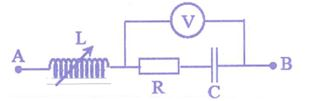
\includegraphics[scale=1]{../figs/VN12-PH-19-P-013-1-6.jpg}
	\end{center}
	\begin{mcq}(4)
		\item $100\ \Omega$.
		\item $60\ \Omega$.
		\item $75\ \Omega$.
		\item $150\ \Omega$.
	\end{mcq}
}	
	\loigiai{
		\textbf{Đáp án: C.}
		
		$Z_C =\dfrac{1}{\omega C} = 100\ \Omega$.
		
		Vôn kế đo hiệu điện thế hai đầu $RC$.
		
		Khi $L$ thay đổi, $U_{RC_\text{max}} \Leftrightarrow I_{\text{max}} $ suy ra trong mạch có cộng hưởng, ta có: $Z=R$.
		
		$$U_{RC_\text{max}} =\dfrac{U}{R} \sqrt{R^2 +Z^2_C} \Rightarrow R =75\ \Omega$$
\item \mkstar{4}

\cauhoi{Trong giờ thực hành, để đo điện dụng $C$ của một tụ điện, một học sinh mắc mạch điện theo sơ đồ như hình bên. Đặt vào hai đầu M,N một điện áp xoay chiều có giá trị hiệu dụng không đổi và tần số $50\ \textrm{Hz}$. Khi đóng khóa K vào chốt 1 thì số chỉ của ampe kế A là $I$. Chuyển khóa K sang chốt 2 thì số chỉ của ampe kế A là $2I$. Biết $R=680\ \Omega$. Bỏ qua điện trở của ampe kế và dây nối. Giá trị của $C$ là
	\begin{center}
		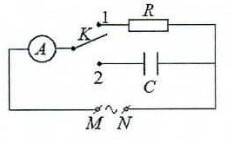
\includegraphics[scale=1.0]{../figs/chap3-6.jpg}
	\end{center}
	\begin{mcq}(2)
		\item $\text{9,36}\cdot 10^{-6}\ \textrm{F}$.
		\item $\text{4,68}\cdot 10^{-6}\ \textrm{F}$.
		\item $\text{18,73}\cdot 10^{-6}\ \textrm{F}$.
		\item $\text{2,34}\cdot 10^{-6}\ \textrm{F}$.
	\end{mcq}		
}		
\loigiai{
	\textbf{Đáp án: A.}
	
		Trường hợp đóng khóa K vào chốt 1, mạch điện gồm có 1 điện trở $R$ mắc vào nguồn điện. 
	Số chỉ của ampe kế cho biết giá trị của cường độ dòng điện hiệu dụng toàn mạch:
	
	$$I=\frac{U}{R}.$$
	Trường hợp đóng khóa K vào chốt 2, mạch điện gồm có 1 tụ điện $C$ mắc vào nguồn điện.
	Số chỉ của ampe kế cho biết giá trị của cường độ dòng điện hiệu dụng toàn mạch:
	
	$$2I=\frac{U}{Z_C}.$$
	
	Từ hai phương trình trên, ta được: 
	
	
	$$\frac {1}{2}=\frac {Z_C}{R} \\ \Leftrightarrow Z_C = \frac {R}{2} \\ \Leftrightarrow \frac {1}{\omega C}= \frac {R}{2} \\ \Leftrightarrow C = \frac {2}{\omega R}=\frac {2}{2\pi fR} \approx \text{9,36}\cdot 10^{-6}\ \textrm{F}.$$
	
}		
		}
	\item \mkstar{3}
	
	\cauhoi{Mạch điện xoay chiều $RLC$ mắc nối tiếp gồm điện trở thuần $R=\SI{10}{\ohm}$, cuộn cảm thuần có cảm kháng $Z_L=\SI{10}{\ohm}$ và tụ điện $C$ có dung kháng $Z_C=\SI{5}{\ohm}$ ứng với tần số $f$. Khi thay đổi tần số dòng điện đến giá trị $f'$ thì trong mạch có cộng hưởng điện. Tần số $f'$ liên hệ với $f$ theo biểu thức
		\begin{mcq}(4)
			\item $f'=f$.
			\item $f=\sqrt{2}f'$.
			\item $f'=\sqrt{2}f$.
			\item $f'=2f$.
		\end{mcq}
}		
		\loigiai{
			\textbf{Đáp án: B.}
			
			Ta có $Z_L=\omega_1L=\SI{10}{\ohm}$; $Z_C=\dfrac{1}{\omega_1 C}=\SI{5}{\ohm}$.
			
			Ta lại có
			$$\dfrac{Z_L}{Z_C}=\omega^2LC=2\Rightarrow \dfrac{\omega^2}{2}=\dfrac{1}{LC}=\omega'^2.$$
			
			Do đó $\omega=\sqrt{2}\omega'\Rightarrow f=\sqrt{2}f'$.
			
		}
	%%%%%%%%%%%%%%CÂU3%%%%%%%%%%
	\item \mkstar{4}
	
	\cauhoi{Đặt điện áp $u=U_0\cos \omega t$  ($U_0$, $\omega$  không đổi) vào đoạn mạch mắc nối tiếp gồm điện trở $R$, tụ điện có điện dung $C$ và cuộn cảm thuần có độ tự cảm $L$ thay đổi. Hình vẽ bên là đồ thị biểu diễn sự phụ thuộc của điện áp hiệu dụng $U_L$ giữa hai đầu cuộn cảm và hệ số công suất $\cos \varphi$  của đoạn mạch theo giá trị của độ tự cảm $L$. Giá trị của $U_0$ gần nhất với giá trị nào sau đây?
		\begin{center}
			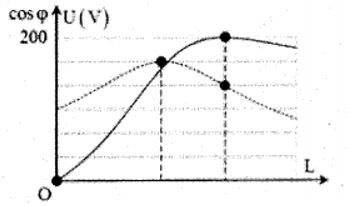
\includegraphics[scale=0.9]{../figs/VN12-PH-19-P-013-1-2.jpg}
		\end{center}
		\begin{mcq}(4)
			\item 240 V.
			\item 165 V.
			\item 220 V.
			\item 185 V.
		\end{mcq}
	}
		\loigiai{
			\textbf{Đáp án: B.}
			
			Khi xảy ra cực đại của điện áp hiệu dụng trên cuộn cảm thuần $$Z_L = \dfrac{R^2+Z^2_C}{Z_C}$$
			
			Ta chuẩn hóa $R=1; Z_C = n \Rightarrow Z_L =\dfrac{1}{x} +x$.
			
			Hệ số công suất của mạch tương ứng $$\cos \varphi =\dfrac{R}{\sqrt{R^2 + (Z_L - Z_C)^2}} \Leftrightarrow \text{0,8} =\dfrac{1}{\sqrt {1+ \dfrac{1}{n^2}}} \Rightarrow n =\dfrac{4}{3}$$
			
			Kết hợp với $$U_{L\text{max}} = U\sqrt {1+ \left (\dfrac{Z_C}{R}\right)^2} \Rightarrow U = \dfrac{U_{L_\text{max}}}{\sqrt {1+\left (\dfrac{Z_C}{R}\right)^2 }} =120\ \text{V}$$
			
			Suy ra $U_0 =120\sqrt 2 \approx 170\ \text{V}$.
			
			
			}
	
	%%%%%%%%%%%%%%CÂU4%%%%%%%%%%

	\item \mkstar{4}
	
	\cauhoi{Cho mạch điện như hình vẽ, hai cuộn dây thuần cảm có độ tự cảm thay đổi, biết $R_2=5R_1$. Đặt vào hai đầu đoạn mạch một điện áp xoay $u =U\sqrt 2 \cos \omega t$ (với $U$ và $\omega$ không đổi). Điều chỉnh độ tự cảm của các cuộn dây (nhưng luôn thoả mãn $L_2=\text{0,8}L_1$) sao cho độ lệch pha giữa điện áp hai đầu đoạn mạch AM và MB lớn nhất, thì hệ số công suất của đoạn mạch khi đó bằng
		\begin{center}
			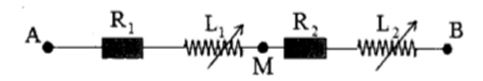
\includegraphics[scale=0.9]{../figs/VN12-PH-19-P-013-1-3.jpg}
		\end{center}
		\begin{mcq}(4)
			\item $\dfrac{8}{\sqrt {73}}$.
			\item 0,8.
			\item 0,6.
			\item $\dfrac{6}{\sqrt {73}}$.
		\end{mcq}
}	
		\loigiai{
			\textbf{Đáp án: A.}
			
			Giản đồ vec tơ như hình 
			\begin{center}
				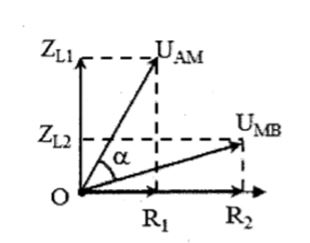
\includegraphics[scale=0.9]{../figs/VN12-PH-19-P-013-1-4.jpg}
			\end{center}
			
			Ta có: $$\tan \alpha = \dfrac {\dfrac{Z_{Z_1}}{R_1} -\dfrac{Z_{L_2}}{R_2}}{1+ \dfrac{Z_{L_1} \cdot Z_{L_2}}{R_1R_2}}$$
			
			Đặt $x = \dfrac{Z_{L_1}}{R_1} \Rightarrow \tan \alpha = \dfrac{\text{0,84}x}{1+\dfrac{\text{0,8}}{5}x^2} = \dfrac {\text{0,84}}{\dfrac{1}{x} +\text{0,16}x}$.
			
			Áp dụng cosi suy ra $\tan \alpha \leq \dfrac{\text{0,84}}{2\sqrt{\text{0,16}}} =\text{1,05}.$
			
			$\Rightarrow \alpha_\text{max} =\text{0,81}$ và $x =\text{2,5}$ hay $Z_{L_1} =\text{2,5}R_1$; $Z_{L_2} =2R_1 \Rightarrow \tan \varphi = \dfrac{Z_{L_1} +Z_{L_2}}{R_1+R_2} =\dfrac{3}{4}$.
			
			$\Rightarrow \cos \varphi = \text{0,8}$.
			
			}
	
	%%%%%%%%%%%%%%CÂU6%%%%%%%%%%
	\item \mkstar{4}
	
	\cauhoi{Đặt một điện áp xoay chiều có giá trị hiệu dụng và tần số không đổi vào hai đầu đoạn mạch điện AB gồm biến trở $R$, tụ điện $C$ và cuộn dây không thuần cảm có độ tự cảm $L$, điện trở thuần $r$, ghép nối tiếp với nhau như hình vẽ.
		\begin{center}
			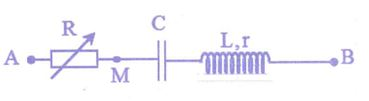
\includegraphics[scale=1]{../figs/VN12-PH-19-P-013-1-5.jpg}
		\end{center}
		Điều chỉnh R đến giá trị $60\ \Omega$ thì công suất tiêu thụ trên biến trở đạt cực đại, đồng thời tổng trở của đoạn mạch AB là số nguyên chia hết cho 45. Khi đó hệ số công suất của đoạn mạch MB có giá trị là
		
		\begin{mcq}(4)
			\item 0,375.
			\item 0,75.
			\item 0,125.
			\item 0,5.
		\end{mcq}
}	
		\loigiai{
			\textbf{Đáp án: C.}
			
			Giá trị của biến trở để công suất tiêu thụ trên biến trở là cực đại:
			
			$$R=R_0 = \sqrt{r^2 +(Z_L-Z_C)^2} = 60\ \Omega$$
			
			+ Tổng trở của mạch khi đó
			
			$$Z= \sqrt{(R_0 +r)^2 +(Z_L-Z_C)^2} = \sqrt {R_0^2 + 2R_0r +r^2 +(Z_L-Z_C)^2} \Rightarrow Z^2 = 60^2 +2 \cdot 60 r + 60^2 = (n \cdot 45)^2 \Rightarrow r =\dfrac{135}{8}n^2 -60$$
			
			+ Hệ số công suất của đoạn mạch MB:
			
			$$\cos \varphi_\text{MB} = \dfrac{r}{\sqrt {r^2 + (Z_L-Z_C)^2 }} = \dfrac{\dfrac{135}{8}n^2 -60}{60}$$
			$$ 0<\cos \varphi_\text{MB} <1 \Leftrightarrow \text{1,89}<n<\text{2,7}$$
			
			$n=2$ suy ra $\cos \varphi_\text{MB} =\text{0,125}$. 
			
			}
	
	%%%%%%%%%%%%%%CÂU7%%%%%%%%%%

	
	%%%%%%%%%%%%%%CÂU8%%%%%%%%%%
	\item \mkstar{4}
	
	\cauhoi{Cho mạch điện như hình vẽ, cuộn dây thuần cảm. Điện áp hai đầu đoạn mạch có biểu thức $u= U\sqrt 2\cos 2\pi f t\ \text{V}$  với $U$ không đổi nhưng $f$ có thể thay đổi được. Ta có đồ thị biểu diễn sự phụ thuộc của công suất tiêu thụ trên mạch theo $R$ là đường liền nét khi $f=f_1$  và là đường đứt nét khi $f=f_2$. Giá trị của $P_\text{max}$  gần nhất với giá trị nào sau đây?
		\begin{center}
			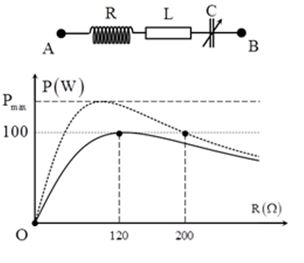
\includegraphics[scale=1.1]{../figs/VN12-PH-19-P-013-1-7.jpg}
		\end{center}
		\begin{mcq}(4)
			\item 280 W.
			\item 140 W.
			\item 130 W.
			\item 260 W.
		\end{mcq}
}		
		\loigiai{
			\textbf{Đáp án: C.}
			
			+	$f=f_1$: Công suất cực đại của mạch khi $R_0 =120 = |Z_{L_1} - Z_{C_1}|.$
			
			Khi đó: $$P_{\text{max}_1} = \dfrac{U^2}{2|Z_{L_1} - Z_{C_1}|} \Rightarrow 100 =\dfrac{U^2}{2 \cdot 120} \Rightarrow U = 40\sqrt {15} \ \text{V}$$
			
			+ $f=f_2$: khi $R=200\ \Omega$ thì công suất tiêu thụ của mạch là 100 W.
			
			$$\Rightarrow 100 = \dfrac{(40\sqrt{15})^2}{200^2 + (Z_{L_2}-Z_{C_2})^2} \cdot 200 \Rightarrow |Z_{L_2}-Z_{C_2}| =40\sqrt 5.$$
			
			Khi đó: $P_\text{max} = P_{\text{max}_2} = \dfrac{U^2}{2|Z_{L_2}-Z_{C_2}|} =60\sqrt 5 \approx \text{134,16}\ \text{W}$.
			
			
			}
	
	%%%%%%%%%%%%%%CÂU9%%%%%%%%%%
	\item \mkstar{4}
	
	\cauhoi{Đặt vào hai đầu đoạn mạch $RLC$ mắc nối tiếp một điện áp xoay chiều có giá trị hiệu dụng và tần số không đổi. Biết $R$ không đổi, cuộn thuần cảm có độ tự cảm $L$ không đổi, điện dung của tụ điện thay đổi được. Khi điện dung $C=C_1$  và $C=C_2$  thì điện áp hiệu dụng hai đầu tụ điện có cùng giá trị, khi $C=C_1$  thì điện áp u hai đầu đoạn mạch trễ pha hơn $i$ một góc $\dfrac{\pi}{6}$. Khi $C=C_2$  thì điện áp $u$ ở hai đầu đoạn mạch trễ pha hơn $i$ một góc $\dfrac{5\pi}{12}$. Khi $C=C_0$  thì điện áp hiệu dụng hai đầu tụ điện đạt giá trị cực đại là $U_{C_\text{max}} = 186\ \text{V}$, đồng thời khi đó điện áp hiệu dụng hai đầu $R$ có giá trị gần nhất với giá trị nào sau đây?
		\begin{mcq}(4)
			\item 200 V.
			\item 100 V.
			\item 180 V.
			\item 150 V.
		\end{mcq}
}		
		\loigiai{
		\textbf{Đáp án: B.}
			
			+ Với $\varphi_1, \varphi_2$ và $\varphi_0$ là độ lệch pha giữa $u$ và $i$ ứng với $C_1; C_2; C_0$.
			
			Ta có: $\varphi_1 + \varphi_2 =2\varphi_0 \Rightarrow \varphi_0 = - \text{52,5}^\circ$.
			
			+ Khi $C=C_0$ điện áp hiệu dụng trên tụ cực đại thì $u_{RL}$ vuông pha với $u$.
			\begin{center}
				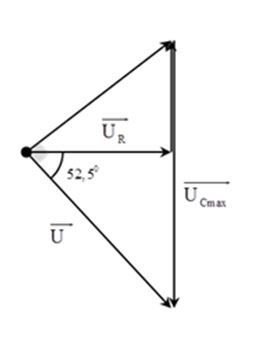
\includegraphics[scale=0.9]{../figs/VN12-PH-19-P-013-1-8.jpg}
			\end{center}
			+ Từ hình vẽ, ta có: 
			
			$$U=U_{C_\text{max}} \sin |\varphi_0|$$
			$$U_R =U \cos |\varphi_0|$$.
			$$\Rightarrow U_R = \dfrac{U_{C_\text{max}}}{2} \sin 2\varphi_0 = 89\ \text{V}$$
			
			
			}
	
	%%%%%%%%%%%%%%CÂU10%%%%%%%%%%
	\item \mkstar{4}
	
	\cauhoi{Cho mạch điện như hình vẽ: $R=100\ \Omega$, cuộn dây thuần cảm có $L=\dfrac{1}{\pi}\ \text{H}$. Khi mắc nguồn điện xoay chiều (100 V - 50 Hz) vào hai điểm A, C thì số chỉ của hai vôn kế như nhau và bằng
		
		\begin{center}
			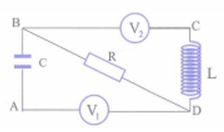
\includegraphics[scale=1.1]{../figs/VN12-PH-19-P-013-1-9.jpg}
		\end{center}
		\begin{mcq}(4)
			\item 141 V.
			\item 100 V.
			\item 200 V.
			\item 150 V.
		\end{mcq}
}	
		\loigiai{
		\textbf{Đáp án: A.}
			
			Sau khi mắc nguồn điện xoay chiều tại hai điểm A và C, mạch điện được vẽ lại như hình trên. 
			
			\begin{center}
				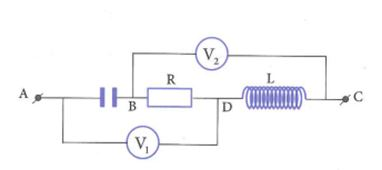
\includegraphics[scale=1.1]{../figs/VN12-PH-19-P-013-1-10.jpg}
			\end{center}
			
			$$U_1 = \sqrt {U_C^2 +U_R^2};U_2 = \sqrt {U_L^2 +U_R^2} (\text{mà} U_1 =U_2) \Rightarrow U_C=U_L.$$ 
			
			Suy ra Mạch đang có cộng hưởng điện nên $U_R=U$.
			$$\Rightarrow I =\dfrac{U}{R} =1\ \text{A}$$.
			$$Z_L = \omega L = 100\ \Omega \Rightarrow U_L = IZ_L = 100\ \Omega$$.
			$$U_{V_1} = U_{V_2} =\sqrt {U^2_L +U^2_R} =100\sqrt 2\ \Omega$$.
		}
\end{enumerate}
\loigiai{\textbf{Đáp án}
	\begin{center}
		\begin{tabular}{|m{2.8em}|m{2.8em}|m{2.8em}|m{2.8em}|m{2.8em}|m{2.8em}|m{2.8em}|m{2.8em}|m{2.8em}|m{2.8em}|}
			\hline
			1. B & 2. A & 3. B & 4. C & 5. D & 6. A  & 7. C  & 8. C & 9. A & 10. B\\
			\hline
			11. A & 12. C & 13. A & 14. A & 15. B & 16. C  & 17. C  & 18. C & 19. A & 20. C\\
			\hline
			21. B & 22. A & 23. A & 24. D & 25. A & 26. B  & 27. A  & 28. D & 29. A & 30. D\\
			\hline
			31. C & 32. C & 33. C & 34. A & 35. B & 36. B  & 37. A  & 38. C & 39. C & 40. B\\
			\hline
		\end{tabular}
\end{center}}